\chapter{Static Single-Assignment}
Dient om eenvoudiger Data-Flow analyse te doen. Maar er moet wel eerst Control-flow analyse gedaan worden.

Er zijn meerdere manieren om te bepalen welke definities van variabalen er bereikbaar zijn in een statement. Op figuur \ref{fig:ssa_example} wordt een voorbeeldprogramma getoond. Men zou de reaching definitions, of nog beter, de use-def chains kunnen bepalen. Maar dit heeft als nadeel dat er verzamelingen van meerdere elementen nog steeds mogelijk zijn.

\begin{figure}[ht]
	\centering
	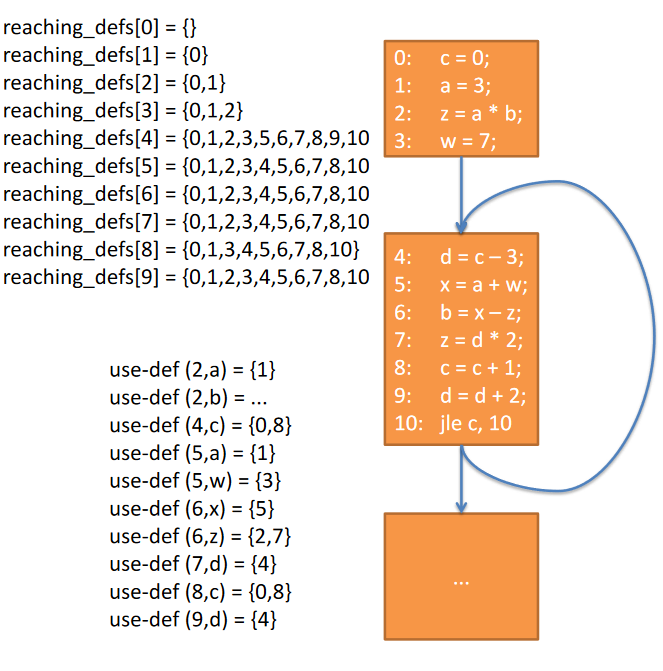
\includegraphics[width=0.7\textwidth]{ssa_example}
	\caption{De reaching definitions en use-def chains van een voorbeeldprogramma.}
	\label{fig:ssa_example}
\end{figure}

In het ideale geval zou elke variabele slechts één definitie heeft, dit wordt Static Single Assignment Form genoemd.

Voordelen:
\begin{itemize}
	\item Slechts 1 def in elke use set.
	\item Elke veranderlijke wordt slechts op 1 plaats in het programma gedefinieerd.
	\begin{figure}[ht]
		\centering
		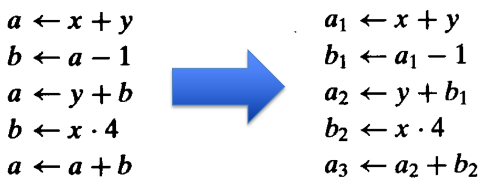
\includegraphics[width=\textwidth]{ssa_example_2}
		\caption{Omvormen programmacode naar SSA.}
		\label{fig:ssa_example_2}
	\end{figure}
	\item De dataverloopanalyse wordt gemakkelijker.
	\item De analyses verlopen nu lineair.
	\item Ontkoppeling veranderlijken met dezelfde naam. De programmeur heeft zelf drie keer de variabele $a$ gebruikt, maar kan even goed andere variabelenamen zijn.
\end{itemize}

In een straight-line programma is het vrij eenvoudig om te omvorming door te voeren. Wanneer conditionele spronge plaatsvinden is het vaak moeilijker. Daarom wordt er een $\phi(a_1, a_2)$-functie geïntroduceerd. De $\phi$-functie in figuur \ref{fig:phi_function} geeft $a_2$ terug als het programma van blok $3$ komt en $a_1$ als het programma van blok $2$ komt. 
\begin{figure}[ht]
	\centering
	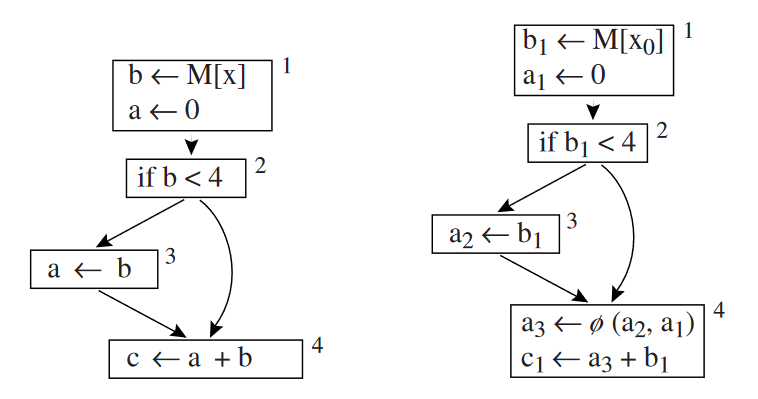
\includegraphics[width=0.7\textwidth]{phi_function}
	\caption{(a) Een programma met controleverloop dat samenkomt; (b) het programma omgezet naar SSA.}
	\label{fig:phi_function}
\end{figure}



Hoe $\phi$-functie wegwerken? Voeg move operaties toe na blok 3 en 2 die respectievelijk $a_2$ en $a_1$ in $a_3$ steken.

Wanneer $\phi$-functie toevoegen?
\begin{itemize}
	\item $a_i$ = $\phi(a_1, ..., a_n)$ is nodig in blok $z$ als
	\begin{itemize}
		\item $a$ gedefinieerd wordt in blok $x$
		\item $a$ gedefinieerd wordt in blok $y \neq x$
		\item Pad van pijlen van $x$ naar $z$ ($P_{xz}$) is niet leeg
		\item Pad van pijlen van $y$ naar $z$ ($P_{yz}$) is niet leeg	
		\item $P_{xz}$ en $P{yz}$ hebben enkel $z$ gemeen
		\item $z$ mag ook midden in $P_{xz}$ of $P_{yz}$ maar niet in beide
		
	\end{itemize}
	\item Wanneer een knoop $x$ een definitie van variabele $a$ bezit, dan moet voor elke knoop $z$ in de dominantiegrens van $x$ een $\phi$-functie aangemaakt worden voor $a$. 

	Een dominantiegrens van een knoop $x$ is een verzameling knopen $w$ waarvoor geldt dat $x$ een predecessor van $w$ domineert maar $w$ zelf niet strikt domineert.
	
	
	Dominantiegrens moet enkel kunnen aangetoond worden op figuur, niet het algoritme kennen.
\end{itemize}




\section{Aggressive Dead Code Elimination}
Eenvoudige variant nadeel: ontdekt geen useless veranderlijken (na sterktereductie)

Aggresieve variant nadeel: stel je stored A in het geheugen (\texttt{STORE A}) Er zijn twee bovenliggende blokken die iets verschillend aan A toekennen. Boven deze twee blokken is er een conditionele jump die bepaald welke van de twee toekenningen uitgevoerd wordt. Er moet ook controleafhankelijkheden bijgehouden worden.